\subsection{Nominator}

\subsubsection{Iterative}
Figure \ref{fig:y-algo:iter} shows a iterative implementation for the
calculation of the nominator.

\begin{figure}[H]
	\centering
	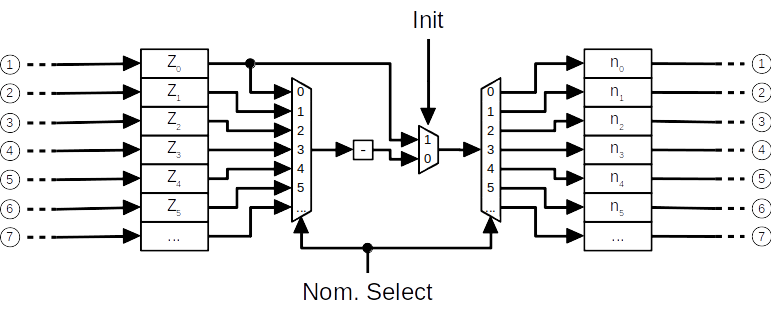
\includegraphics[width=.8\textwidth]{content/results/y-algo_iterative.png}
	\caption{Hardware algorithm to calculate the denominator consecutively.}
	\label{fig:y-algo:iter}
\end{figure}

Because of the triangular nature of the recursion, shown in table 6, the
register will hold the coefficients at the end of the computation reducing the
number of registers needed as the result does not have to be stored separately.

This implementation might prove to be to slow as the number of iterations is
proportional to $\frac{n^2}{2}$.



\subsubsection{Parallelization}
This implementation can easily parallelized to a certain extent to reduce the
quadratic nature to a linear nature. Figure \ref{fig:y-algo:parallel} shows a
parallelized version of the implementation.

\begin{figure}[H]
	\centering
	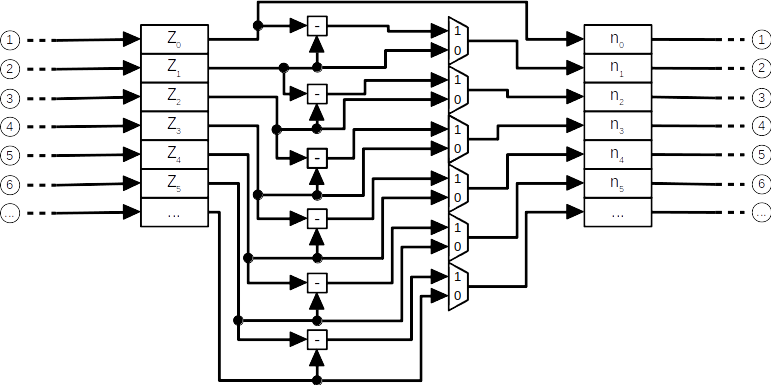
\includegraphics[width=.8\textwidth]{content/results/y-algo_parallel.png}
	\caption{Hardware algorithm to calculate the denominator with
		lookup-table for non-normed intervals.}
	\label{fig:y-algo:parallel}
\end{figure}
